\section{Teoria}

\subsection{Máquina de Estado Finito}

Máquinas de estado finito (MEF) são o tipo mais simples e restrito de autômato,
capazes apenas de processar linguagens do tipo 3: ``gramática regular'',
geradas por expressões regulares.

Uma MEF pode ser considerada como um modelo simplificado do funcionamento de um
computador. Esta pode ser definida como uma quíntupla ordenada $M = (S, I, O,
f_S, f_O)$ onde:
\begin{itemize}
    \item $S$ é o conjunto finito de estados;
    \item $I$ é o conjunto finito de símbolos de entrada (alfabeto de entrada);
    \item $O$ é o conjunto finito de símbolos de saída (alfabeto de saída);
    \item $f_S: S \times I \rightarrow S$ é uma função que retorna o próximo
          estado $s_{t_{k+1}} \in S$ dado o estado anterior $s_{t_k} \in S$ e
          um símbolo de entrada $i_{t_k} \in I$;
    \item $f_O: S \rightarrow O$ é a função \textit{output}, que retorna o
          símbolo de saída $o_{t_k} \in O$ do estado atual $s_{t_k} \in S$.
\end{itemize}

As operações da MEF são sincronizadas por pulsos discretos de um relógio
(\textit{clock}) representados por $t_k$, onde $k \in \mathbb{N}_0$ representa o
ciclo de \textit{clock} atual. Partindo de um estado inicial $s_0 = s_{t_0}$,
após um pulso de \textit{clock}, a função $f_S$ retornará um novo estado
$s_{t_1}$ dado a entrada anterior $i_{t_0}$ e o estado anterior $s_0$.
Generalizando para qualquer pulso de \textit{clock}, é possível afirmar que a
MEF possui um comportamento determinístico, ou seja, o novo estado sempre
dependará do estado e entrada anteriores. Cada estado funciona como uma memória
dos \textit{inputs} anteriores, além de possuir um símbolo de saída, que é
retornado pela função \textit{output} $f_O$.

\begin{figure}[H]
    \centering
    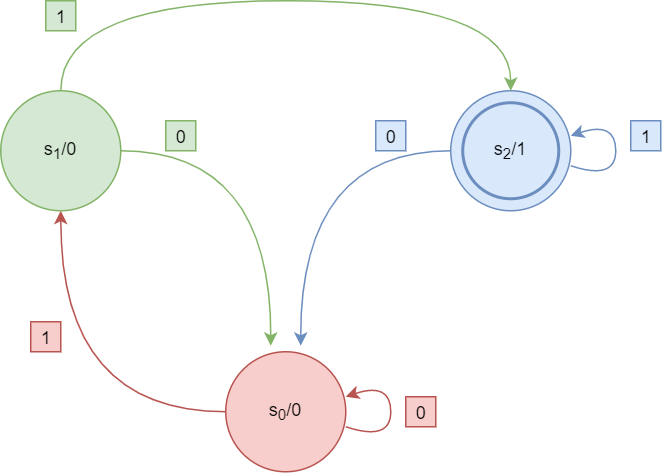
\includegraphics[width=0.7\textwidth]{fsm}
    \caption{Exemplo de máquina de estado finito}
    \label{fig:fsm}
\end{figure}

Tomando como exemplo a MEF acima, começamos no estado $s_0$ e temos como saída o
símbolo \textbf{0}. Aqui, há duas possibilidades: enquanto a entrada for
\textbf{0}, permanecemos neste estado; caso a entrada seja \textbf{1}, seguimos
para o estado $s_1$. Ao seguirmos para o estado $s_1$, temos como saída o
símbolo \textbf{0}. Novamente, há duas possíveis entradas: caso a entrada seja
\textbf{0}, retornamos ao estado $s_0$; caso a entrada seja \textbf{1}, seguimos
para o estado $s_2$. Por fim, ao seguirmos para o estado $s_2$, temos como saída
o símbolo \textbf{1}. As alternativas são: caso a entrada seja \textbf{0},
retornarmos ao estado $s_0$; enquanto a entrada seja \textbf{1}, permanecemos
neste estado.

Esta forma um tanto verbosa de se descrever uma MEF pode ser colocada em uma
tabela, com o estado atual, possíveis entradas e saídas como colunas da mesma.

\begin{table}[H]
    % https://tex.stackexchange.com
    % /questions/192842/multiple-columns-in-table-problem-with-alignment
    % Use `L{width}', `C{width}' or `R{width}' for column alignment
    \centering
    \begin{tabular}{ c C{1cm} C{1cm} c }
        \toprule
        Estado Atual & \multicolumn{2}{c}{Próximo Estado} & Saída      \\
                     & \textbf{0} & \textbf{1}            &            \\
        \hline
        $s_0$        & $s_0$      & $s_1$                 & \textbf{0} \\
        $s_1$        & $s_0$      & $s_2$                 & \textbf{0} \\
        $s_2$        & $s_0$      & $s_2$                 & \textbf{1} \\
        \bottomrule
    \end{tabular}
    \caption{Tabela de estados da MEF representada na Fig.\ \ref{fig:fsm}}
    \label{tab:fsm}
\end{table}

Nota-se que dentre todas as possíveis entradas, esta MEF só aceitará, isto é,
terminará no estado final $s_2$, para \textit{strings} de entrada que terminem
com dois ou mais \textbf{1} (\textbf{11}, \textbf{111}, \textbf{1111}, \ldots).

\subsection{Máquina de Turing}

Máquinas de estado finito são capazes de processar apenas gramáticas do tipo 3:
``gramática regular''. Sendo assim é necessário o uso de outros tipos de
autômatos para o processamento de gramáticas do tipo 2, 1 e 0: ``livre de
contexto'', ``sensível ao contexto'' e ``recursivamente enumerável'',
respectivamente.

Segundo a hierarquia de Chomsky, cada classe de gramática é um superconjunto da
gramática anterior. Sendo assim, a gramática mais geral, a ``recursivamente
enumerável'' com o seu respectivo autômato, a máquina de Turing, é capaz de
representar e processar linguagens formais de qualquer outra classe.

A máquina de Turing (MT), criada por Alan Turing \cite{turing}, é o modelo mais
geral do
funcionamento de um
computador. Considera-se uma fita de comprimento infinito que armazena os dados
de entrada da MT. Cada dado ocupa uma posição da fita. Anexado a esta fita, há
um cabeçote, que pode ler e escrever dados da fita sob a posição em que se
encontra. Este pode mover-se para a esquerda e para direita apenas uma posição
por vez. O cabeçote serve como dispositivo de entrada/saída da MT.

\begin{figure}[H]
    \centering
    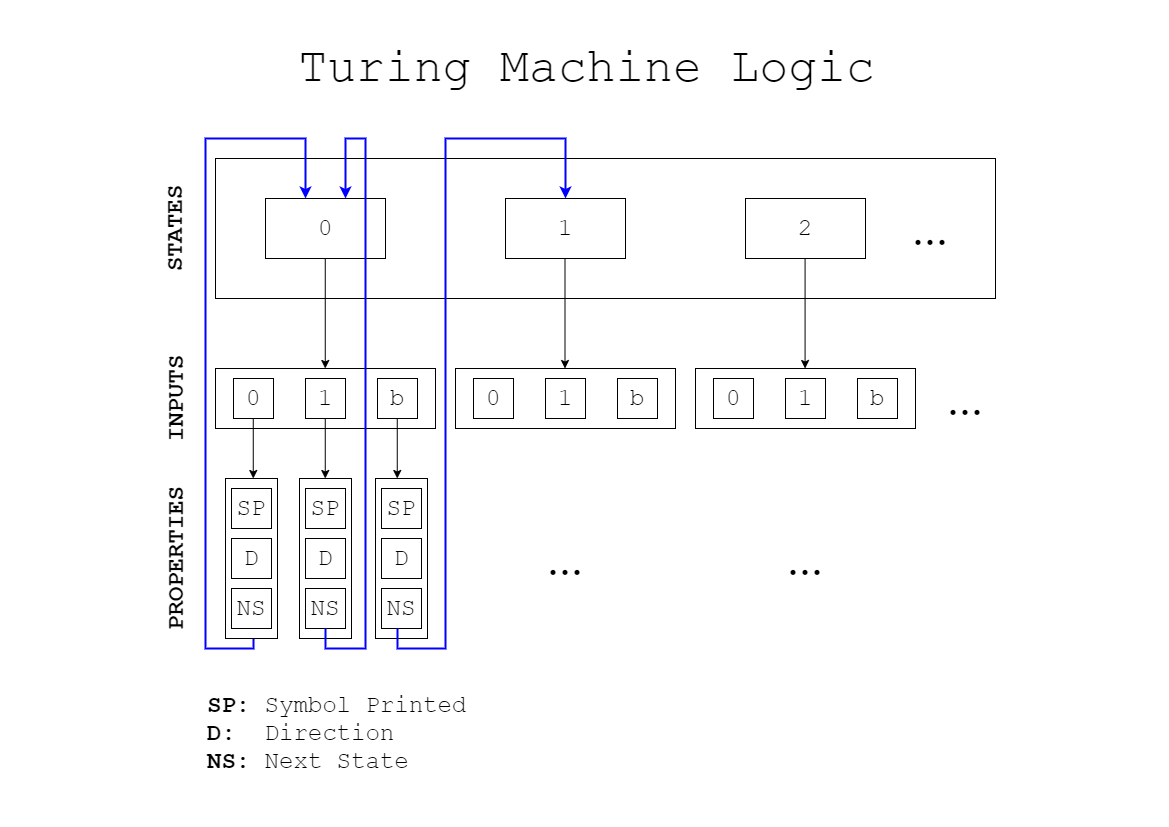
\includegraphics[width=0.9\textwidth]{tm}
    \caption{Elementos da máquina de Turing}
    \label{fig:tm}
\end{figure}

Para um conjunto finito de estados $S$ e para um conjunto finito de símbolos da
fita (alfabeto da fita) $I$, define-se uma MT como uma quíntupla ordenada $T =
(s, i, i', s', d)$ onde:
\begin{itemize}
    \item $s \in S$ é o estado da MT;
    \item $i \in I$ é um símbolo de entrada;
    \item $i' \in I$ é um símbolo de saída;
    \item $s' \in S$ é o novo estado da MT;
    \item $d \in \{L,R\}$ é direção de movimento do cabeçote.
\end{itemize}

Para cada dado $i$ lido pela MT, dado o estado atual $s$, resultará em uma
saída $i'$, um novo estado $s'$ e uma direção de movimento do cabeçote $d$.
Nota-se que exceto pelo componente $d$, a MT é idêntica a MEF, mas devido a
fita com capacidade de memória infinita e a possibilidade de ler e escrever e
reler os dados da própria fita, faz com que a MT seja de processar gramáticas
que seriam impossíveis em uma MEF.

\section{Desenvolvimento}

Tendo a teoria como base, foi possível escrever uma implementação computacional
destes autômatos. A linguagem escolhida foi \textit{Python}, pois sua
orientação a objetos e simplicidade de sintaxe permitiu uma modelagem do
problema de forma mais direta, rápida e eficiente.

\subsection{Máquina de Estado Finito}

A máquina de estado finito foi implementada como uma classe (\verb|FSM|), onde
seus estados estão armazenados em uma lista, e cada estado nesta lista é um
dicionário com chaves correspondentes ao próprio estado (\verb|state|),
próximo estado se o \textit{input} for \textbf{0} (\verb|next0|), próximo
estado se o \textit{input} for \textbf{1} (\verb|next1|) e ao \textit{output}
(\verb|output|), nesta ordem. Esta abordagem foi tomada para facilidade de
interpretação do código; ao invés de utilizar apenas índices, o uso das chaves
nomeadas torna o funcionamento mais explícito.

Esta lista de dicionários é preenchida a partir da leitura de um arquivo
\verb|.yaml|, onde o usuário pode configurar os estados da MEF.

Ao iniciar o programa, o mesmo realiza a inicialização de uma instância da MEF,
e em seguida pede ao usuário a inserção de um \textit{string} de entrada. Ao
pressionar \keys{\return}, esta \textit{string} é processada pela MEF, e, para
cada símbolo de entrada, o estado interno é atualizado, e o símbolo de saída
correspondente é impresso no console. Após todos os símbolos terem sido
processados, o programa solicita ao usuário uma nova \textit{string} de entrada.
Para encerrar a execução do programa, o usuário pode usar o atalho de teclado
\keys{\ctrl+C} ou \keys{\ctrl+D}.

\begin{figure}[H]
    \centering
    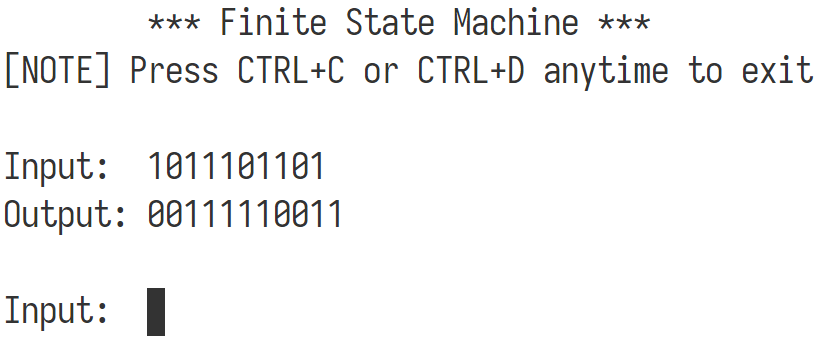
\includegraphics[width=0.8\textwidth]{fsm_run}
    \caption{Execução da máquina de estado finito}
    \label{fig:fsm_run}
\end{figure}

Caso uma \textit{string} contenha símbolos diferentes de \textbf{0} ou
\textbf{1}, uma mensagem de erro é mostrada e o programa encerra sua execução.

\subsection{Máquina de Turing}

A máquina de Turing foi implementada como duas classes: uma para a lógica do
programa (\verb|TuringMachine|), e a outra para a fita (\verb|Tape|).

Na classe \verb|TuringMachine|, as quíntuplas da MT, são armazenadas em um
dicionário, onde cada elemento do dicionário corresponde a um estado, cada
estado é um dicionário que contém os símbolos de entrada, e cada símbolo de
entrada é um dicionário que contém a própria quíntupla, isto é, estado atual
(\verb|present_state|), símbolo de entrada (\verb|present_symbol|), símbolo de
saída \linebreak (\verb|symbol_printed|), direção (\verb|direction|) e o próximo
estado (\verb|next_state|).

\begin{figure}[H]
    \centering
    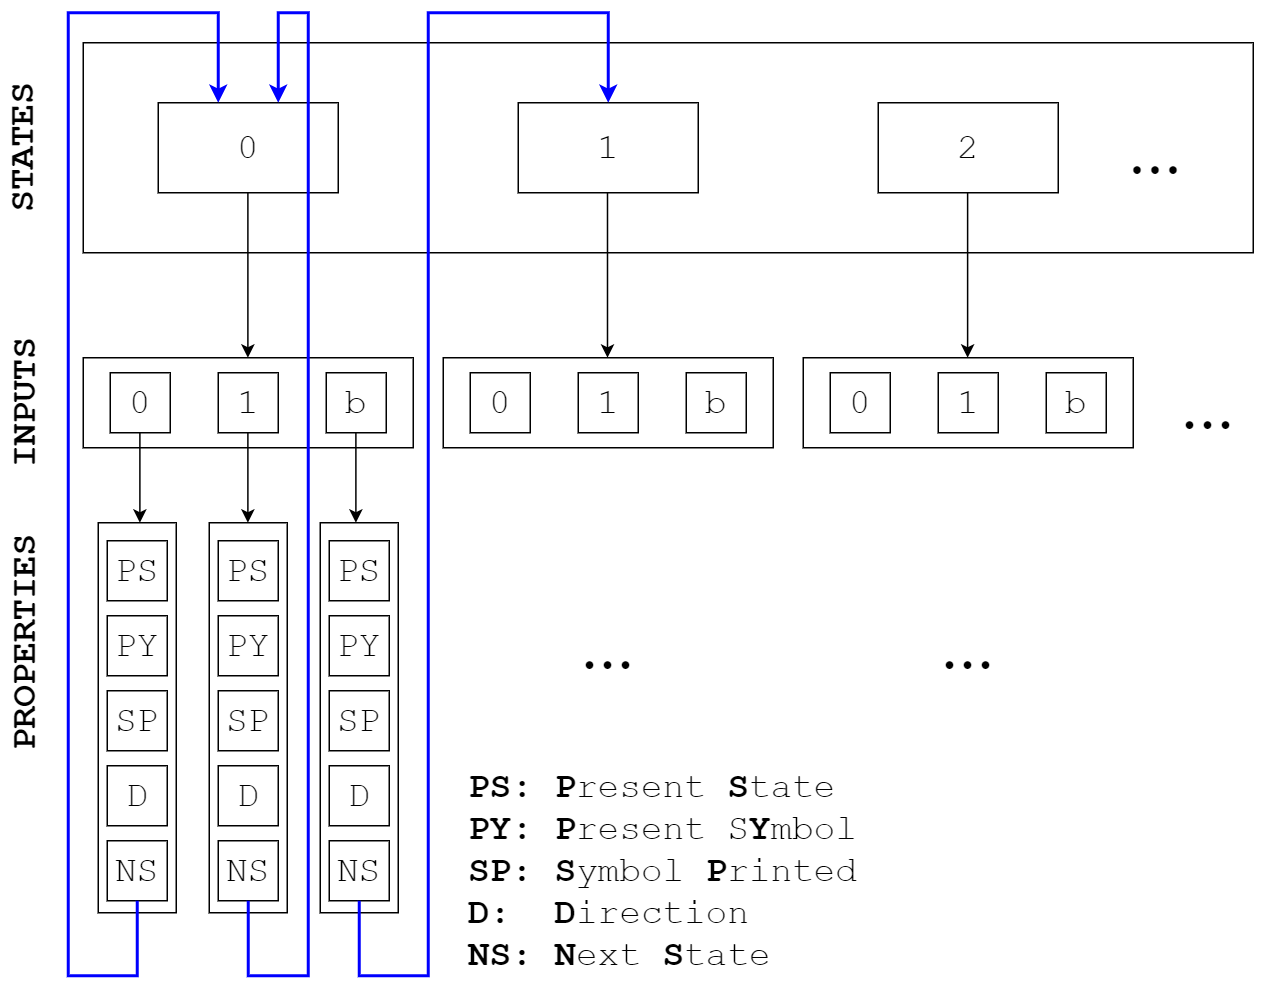
\includegraphics[width=0.8\textwidth]{tm_logic}
    \caption{Lógica de funcionamento da máquina de Turing}
    \label{fig:tm_logic}
\end{figure}

A essência do funcionamento da MT é apresentada na figura acima, onde, para um
dado estado, dependendo do símbolo de \textit{input}, pode-se ter diferentes
símbolos de \textit{output}, direções e próximos estados.

Na classe \verb|Tape|, a fita é implementada como uma lista de comprimento 70,
que será preenchida com a \textit{string} de entrada.

Tanto o dicionário de quíntuplas quanto os dados de entrada da fita são
preenchidos a partir da leitura de um arquivo \verb|.yaml|, onde o usuário pode
configurar os parâmetros da MT.

Ao iniciar o programa, o mesmo realiza a inicialização de instâncias da MT e da
fita, e exibe no console uma mensagem de confirmação: caso o usuário pressione
\keys{\enter}, a execução da MT é iniciada, caso o usuário pressione
\linebreak \keys{\ctrl+C} ou \keys{\ctrl+D}, o programa é encerrado. Partindo do
pressuposto que o usuário decidiu iniciar a execução, o programa irá mostrar no
console uma representação visual da fita, os dados nela presentes, e do cabeçote
de leitura e escrita.

\begin{figure}[H]
    \centering
    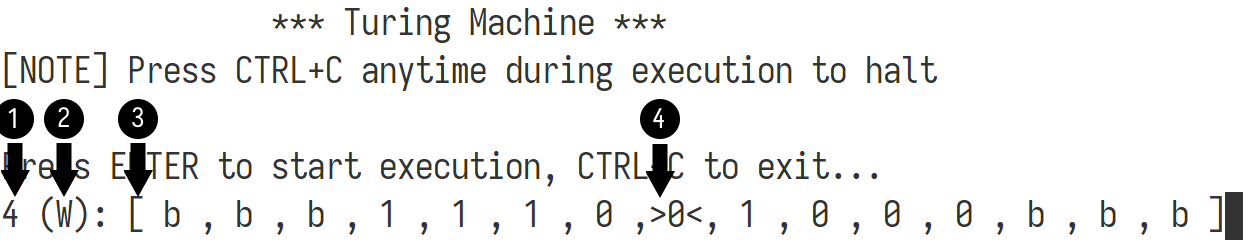
\includegraphics[width=\textwidth]{tm_run}
    \caption{Execução da máquina de Turing}
    \label{fig:tm_run}
\end{figure}

Os seguintes elementos podem ser vistos nesta imagem:

\begin{enumerate}
    \item Iteração atual;
    \item Ação atual do cabeçote (Leitura (\verb|R|) ou Escrita (\verb|W|));
    \item Fita e seu conteúdo;
    \item Posição atual do cabeçote (representado pelo par \verb|> <|).
\end{enumerate}

A cada iteração o cabeçote realiza uma etapa de leitura e uma etapa de escrita.
Durante a leitura, o símbolo lido é comparado com os símbolos de \textit{input}
para aquele estado. Em seguida, o símbolo de \textit{output} é escrito, a MT
assume o novo estado, e o cabeçote se move em uma nova direção. Caso o próximo
estado não exista, ou o símbolo de entrada não consta dentre os \textit{inputs}
do estado atual, o programa encerrará a sua execução.

Devido a impossibilidade de se determinar para quais conjuntos de entradas e
quíntuplas a MT irá concluir sua execução ou ficará em um \textit{loop} infinito
(Halting Problem \cite{turing}), é possível estabelecer um número máximo de
iterações para a MT através de um parâmetro no arquivo \verb|.yaml|. Caso o
usuário deseje, este também pode parar a execução do programa a qualquer
momento, pressionando \linebreak \keys{\ctrl+C}.

Devido aos limites físicos de um computador real em relação à MT teórica --- no
caso, memória finita --- caso o cabeçote passe dos limites da fita (estabelecido
como 70), a execução do programa será encerrada.

\section{Resultados}

Com o desenvolvimento do código concluído, testes foram realizados para
verificar a acurácia das soluções obtidas.

\subsection{Máquina de Estado Finito}

Os testes foram realizados a partir de exemplos extraídos do livro
\cite[cap.\ 9.3]{judith}.

\subsubsection*{p.\ 730, Example 29:}

\begin{table}[H]
    % https://tex.stackexchange.com
    % /questions/192842/multiple-columns-in-table-problem-with-alignment
    % Use `L{width}', `C{width}' or `R{width}' for column alignment
    \centering
    \begin{tabular}{ c C{1cm} C{1cm} c }
        \toprule
        Estado Atual & \multicolumn{2}{c}{Próximo Estado} & Saída      \\
        & \textbf{0} & \textbf{1}            &            \\
        \hline
        $s_0$        & $s_1$      & $s_0$                 & \textbf{0} \\
        $s_1$        & $s_2$      & $s_1$                 & \textbf{1} \\
        $s_2$        & $s_2$      & $s_0$                 & \textbf{1} \\
        \bottomrule
    \end{tabular}
    \caption{\cite[p.\ 730, Example 29 --- Table 9.1]{judith}}
    \label{tab:fsm_chap9.3_ex29}
\end{table}
\begin{figure}[H]
    \centering
    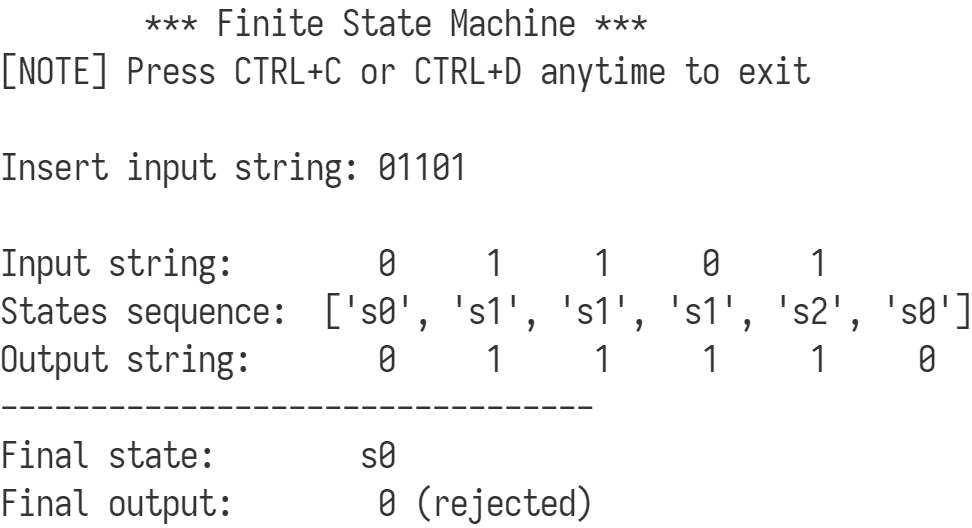
\includegraphics[width=0.7\textwidth]{fsm_chap9.3_ex29}
    \caption{
        \textit{Output} da MEF definida na Tabela \ref{tab:fsm_chap9.3_ex29}
        para o \textit{input} proposto pelo ``Example 29''
    }
    \label{fig:fsm_chap9.3_ex29}
\end{figure}

\subsubsection*{p.\ 731, Practice 43:}

``For the machine \textit{M} of Example 29, what output sequence is produced by
the input sequence 11001?''
\begin{figure}[H]
    \centering
    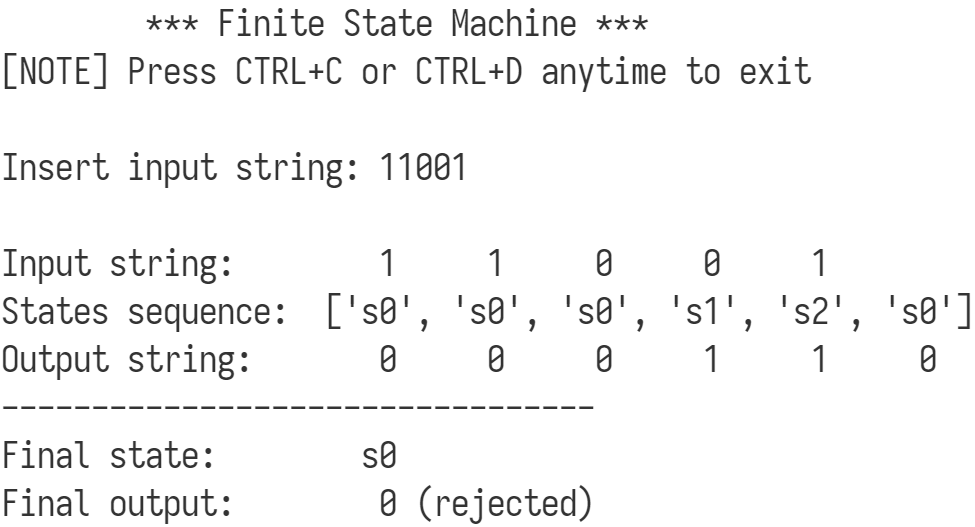
\includegraphics[width=0.7\textwidth]{fsm_chap9.3_prac43}
    \caption{
        \textit{Output} da MEF definida na Tabela \ref{tab:fsm_chap9.3_ex29}
        para o \textit{input} proposto pela questão ``Practice 43''
    }
    \label{fig:fsm_chap9.3_prac43}
\end{figure}

%%%%%%%%%%%%%%%%%%%%%%%%%%%%%%%%%%%%%%%%%%%%%%%%%%%%%%%%%%%%%%%%%%%%%%%%%%%%%%%%
\begin{center}
    \hrule
    <Inserir mais exemplos>
    \hrule
\end{center}
%%%%%%%%%%%%%%%%%%%%%%%%%%%%%%%%%%%%%%%%%%%%%%%%%%%%%%%%%%%%%%%%%%%%%%%%%%%%%%%%

\subsection{Máquina de Turing}

Os testes foram realizados a partir de exemplos extraídos do livro
\cite[cap.\ 9.4]{judith}, exceto quando indicado.

\subsubsection*{p.\ 762, Example 40:}

% Side-by-side
\begin{table}[H]
    \begin{minipage}{0.666\linewidth}

        \begin{minipage}{.5\linewidth}
            Quíntuplas da máquina:
        \end{minipage}% <-- This comment fixes aligment, do not remove
        \begin{minipage}{.5\linewidth}
            \ttfamily
            (0, 0, 1, 0, R) \\
            (0, 1, 0, 0, R) \\
            (0, b, 1, 1, L) \\
            (1, 0, 0, 1, R) \\
            (1, 1, 0, 1, R)
        \end{minipage}

    \end{minipage}% <------ This comment fixes aligment, do not remove
    \begin{minipage}{0.333\linewidth}

       \begin{flushright}
            \textit{String} de entrada: \textbf{0110}
       \end{flushright}

    \end{minipage}

    \caption{\cite[p.\ 762, Example 40]{judith}}
    \label{tab:tm_chap9.4_ex40}
\end{table}

\begin{figure}[H]
    \centering
    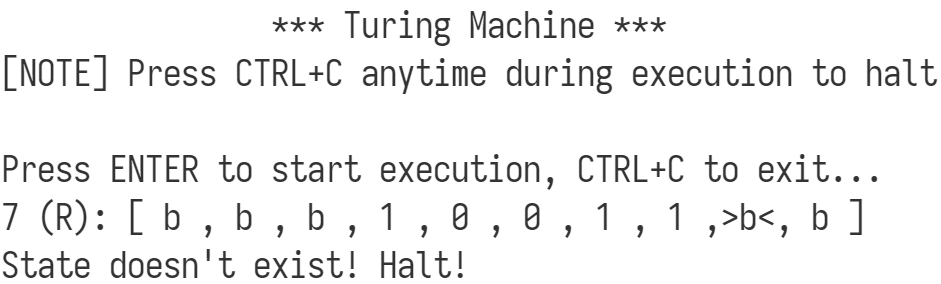
\includegraphics[width=0.8\textwidth]{tm_chap9.4_ex40}
    \caption{
        Estado final da fita após a finalização da execução da MT definida na
        Tabela \ref{tab:tm_chap9.4_ex40}
    }
    \label{fig:tm_chap9.4_ex40}
\end{figure}

\subsubsection*{p.\ 764, Practice 57:}

% Side-by-side
\begin{table}[H]
    \begin{minipage}{.5\linewidth}
        \begin{flushright}
            Quíntuplas da máquina:\hspace*{1ex}    % Add unremovable space @ EOL
        \end{flushright}
    \end{minipage}% <-- This comment fixes aligment, do not remove
    \begin{minipage}{.5\linewidth}
            \ttfamily
            \hspace*{1ex}(0, 0, 0, 1, R) \\        % Add unremovable space @ SOL
            \hspace*{1ex}(0, 1, 0, 0, R) \\        % Add unremovable space @ SOL
            \hspace*{1ex}(0, b, b, 0, R) \\        % Add unremovable space @ SOL
            \hspace*{1ex}(1, 0, 1, 0, R) \\        % Add unremovable space @ SOL
            \hspace*{1ex}(1, 1, 1, 0, L)           % Add unremovable space @ SOL
    \end{minipage}

    \caption{\cite[p.\ 764, Practice 57]{judith}}
    \label{tab:tm_chap9.4_prac57}
\end{table}

\begin{enumerate}[a.]
    \item \textit{String} de entrada: \textbf{10}
\end{enumerate}

\begin{figure}[H]
    \centering
    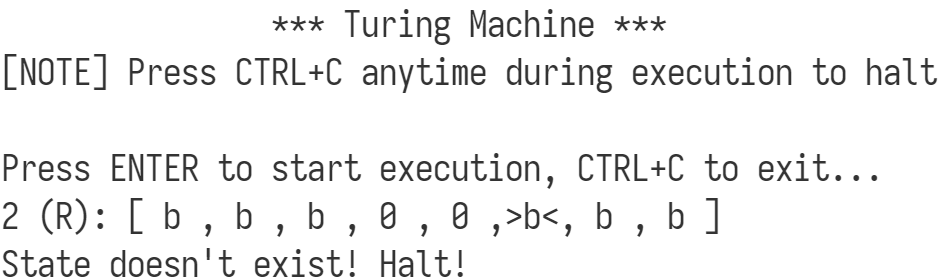
\includegraphics[width=0.8\textwidth]{tm_chap9.4_prac57a}
    \caption{
        Estado final da fita após a finalização da execução da MT definida na
        Tabela \ref{tab:tm_chap9.4_prac57} para o \textit{input} \textbf{10}
    }
    \label{fig:tm_chap9.4_prac57a}
\end{figure}

\begin{enumerate}[resume*]
    \item \textit{String} de entrada: \textbf{01}
\end{enumerate}

Para esta \textit{string} de entrada, a máquina fica presa em um \textit{loop},
sendo necessário a parada manual de sua execução (\keys{\ctrl+C}). Mesmo assim,
a fita alcança um estado final, após o qual os seus dados não são mais
alterados.

\begin{figure}[H]
    \centering
    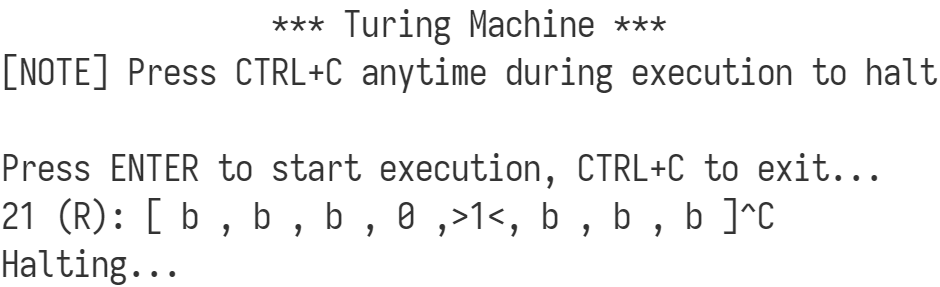
\includegraphics[width=0.8\textwidth]{tm_chap9.4_prac57b}
    \caption{
        Estado da final fita após parada manual da execução da MT definida na
        Tabela \ref{tab:tm_chap9.4_prac57} para o \textit{input} \textbf{01}
    }
    \label{fig:tm_chap9.4_prac57b}
\end{figure}

\begin{enumerate}[resume*]
    \item \textit{String} de entrada: \textbf{00}
\end{enumerate}

Para esta \textit{string} de entrada, o cabeçote começa a se mover para a
direita sem fim. Devido aos limites físicos da fita previamente estabelecidos,
ao alcançar a extremidade direita, a execução é abortada. Apesar disso, após
certo ponto, os dados da fita não são alterados.

\begin{figure}[H]
    \centering
    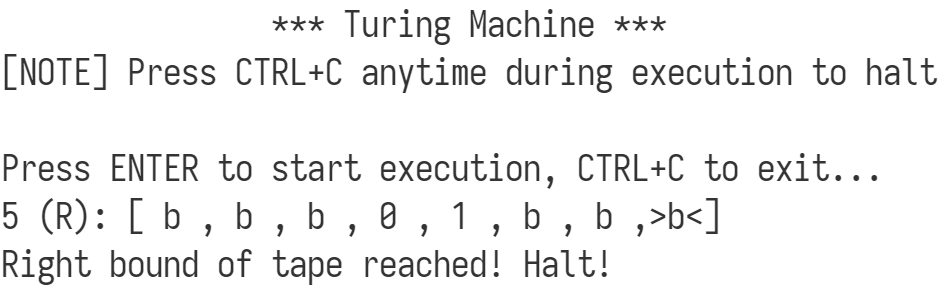
\includegraphics[width=0.8\textwidth]{tm_chap9.4_prac57c}
    \caption{
        Estado da final fita após parada da execução da MT definida na
        Tabela \ref{tab:tm_chap9.4_prac57} ao ultrapassar a extremidade direita
        para o \textit{input} \textbf{00}
    }
    \label{fig:tm_chap9.4_prac57c}
\end{figure}

\subsubsection*{Exemplo Próprio}

Para demonstrar mais uma peculiaridade no funcionamento de uma MT, abaixo segue
um esquema próprio.

% Side-by-side
\begin{table}[H]
    \begin{minipage}{0.6\linewidth}

        \begin{minipage}{0.55\linewidth}
                Quíntuplas da máquina:
        \end{minipage}% <-- This comment fixes aligment, do not remove
        \begin{minipage}{0.45\linewidth}
            \ttfamily
            (0, 0, 1, 0, R) \\
            (0, 1, 0, 0, R) \\
            (0, b, b, 1, L) \\
            (1, 1, 0, 1, L) \\
            (1, 0, 1, 1, L) \\
            (1, b, b, 0, R)
        \end{minipage}

    \end{minipage}% <------ This comment fixes aligment, do not remove
    \begin{minipage}{0.4\linewidth}

        \begin{flushright}
            \textit{String} de entrada: \textbf{000111000}
        \end{flushright}

    \end{minipage}

    \caption{Exemplo Próprio de MT}
    \label{tab:tm_own_ex}
\end{table}

Para a MT acima, o seu comportamento independe da string de entrada. Dado que
não seja vazia (\textbf{b}), a mesma ficará presa em um \textit{loop} infinito,
reescrevendo \textbf{0} em \textbf{1} e \textbf{1} em \textbf{0}, até alcançar
um \textbf{b}; após esse ponto, a mesma reverte a direção e desfaz as
alterações. Ao alcançar outro \textbf{b}, ela novamente reverte de direção e
o processo se repete.

\begin{figure}[H]
    \centering
    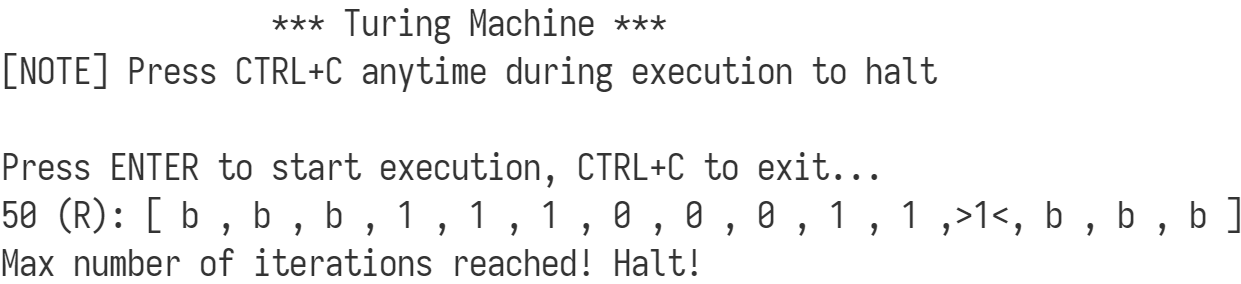
\includegraphics[width=\textwidth]{tm_own_ex_50i}
    \caption{
        Estado da fita após parada da execução da MT definida na
        Tabela \ref{tab:tm_own_ex} ao alcançar um número máximo de iterações
        (50) para o \textit{input} \textbf{000111000}
    }
    \label{fig:tm_own_ex_50i}
\end{figure}